% Copyright (C) 2019 Cui Jialiang ( SESS, PKU ). All rights reserved.

\chapter{基于Tensorflow的像素级视频目标跟踪实验}
为了验证本研究提出的方法的可行性和价值,我们设计了一个实验。后文中该实验将被称为本实验。本实验基本实现了本研究提出的方法,并得到了一定的结果和结论.
\par
本章接下来的部分将介绍本实验的设计思路,硬件环境和数据等实验条件,实验代码的实现和实验结果的评估方法。

\section{实验总体设计思路}
类似于大多数算法研究,本研究以计算机软件的形式实现了本研究提出的算法,并选择数据进行了实验.

\section{实验软硬件环境}
\subsection{软件环境}
本实验的软件部分主要在Tensorflow\supercite{abadi2016tensorflow}框架下实现。
\par
Tensorflow是最初由谷歌公司开发的一套现以开源的机器学习框架,可以为算法研究者提供屏蔽操作系统与硬件,资源分配,梯度计算等功能,让研究者能将更多的注意力集中在算法过程中.对于本研究,Tensorflow主要贡献了CNN,RNN单元的结构定义,损失函数定义,正向反向传播与梯度更新等功能.

\subsection{硬件环境}
\par
需要说明的是本研究提出的算法可以部署在普通计算机上,也有希望部署在更快速,更低成本的FPGA等嵌入式平台上.本实验为了容易进行,目前只在PC(个人计算机)上进行.
\par
本实验所有的运算操作是在一台配置有英伟达GTX1070图形处理器,英特尔i7中央处理器,24GB内存的笔记本电脑上进行的。
\par
本实验深度学习计算部分使用了GPU加速,直接依赖Tensorflow的GPU选项进行。本研究曾尝试过只用CPU进行计算,也能得到一定结果。
\par
如果有更好的硬件条件(更多、更好的图形处理器,更大的内存,更多核心的CPU),本实验有希望会得到更精细的结果。

\section{实验数据}
本实验使用VOT2016数据集\supercite{Vojir-TR-2017-01}实现,相似的数据集还有VOT2017等。
\par
\begin{figure}[htbp!]
    \centering
    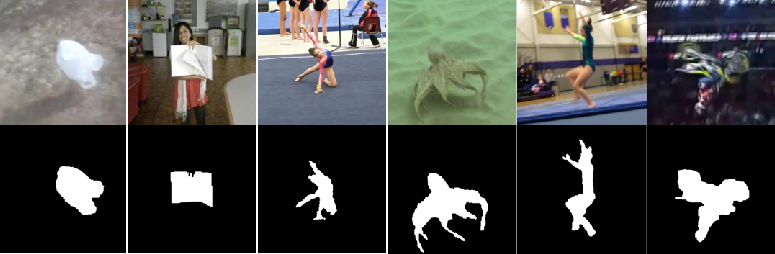
\includegraphics[width = 1.\textwidth]{chap/img/vot_2016_pixel.png}
    \caption{VOT2016像素级标记}\label{fig:vot_2016_pixel}
\end{figure}
\par
如图\ref{fig:vot_2016_pixel}所示,该数据集通过人工标记,提供了十分优秀的像素级的目标跟踪数据。该数据集有几百个序列,共有几万张图片。
\par
本实验的训练集和测试集均来源于该数据集,使用时将所有数据随机切分为训练集和测试集。
\subsection{Ground truth}
Ground truth是一个机器学习中的概念,意为根据某种参考得到的标注数据.尤其是在图像领域,所有的参考都不能被肯定是完全正确的,ground truth就指这样的标注结果.大多数ground truth可以有很强的正确性,如大多数人工标注的图像训练数据,其正确程度已经可以用于机器学习训练,但在一些边界区域还是会有一些人工操作导致的误差.

\section{实验程序的编写}
事实上,虽然借助于Tensorflow实现了许多计算功能,但本研究依然经历了许多代码开发工作,包括且不限于神经网络结构定义,训练数据处理等.
\par
本实验现先定义了CRNN的结构,即输入一个时间序列的序列图像,经过CRNN卷机循环网络得到另一个结果时间序列.在本实验的程序中,该结构可以选择使用LSTM或普通RNN单元.
\par
在加密-解码结构中,本实验定义了一个通用的层级结构,可以重复使用多次.如重复3次即是3层加密-解码结构.

\section{实验结果的评估方式}
由于像素级的视频目标跟踪算法缺乏评估体系,本实验直接将跟踪问题视为像素级二分类问题,用二分类问题的评价方式来评价实验结果.
\par
% TODO 混淆矩阵
对于像素级跟踪问题,分类结果中所有像素可以分为分类得到的正例(目标)和负例(背景),同样的,ground truth中标记的像素也可以分为正例和负例.
\par
对于ground truth中标记为正例和负例的像素,分别被分成正例和负例可以用混淆矩阵表示.

\subsection{分类问题评估:准确率和召回率}
准确率(accuracy)和召回率(recall)可以用于描述分类问题的精确程度.
\par
准确率指分类器将结果分对的概率,将正例分为正例,将负例分为负例都是分对.在本实验中,准确率可以衡量一个跟踪算法大体上对结果的正确估计率.但如果在一个场景中目标较小,将所有像素分为背景的算法依然能得到很高的准确率.
\par
\begin{equation}\label{equ:accuracy}  Accuracy=\frac{TP+TN}{TP+FP+TN+FN}  \end{equation}
\par
召回率指正例结果的正确性,即结果中的正结果,其是本来就是正例的概率.该衡量方式避免了准确率带来的问题,但只能估计目标,无法确定背景的预测准确定.
\par
\begin{equation}\label{equ:recall}  Recall=\frac{TP}{TP+FN}  \end{equation}
\par
上述准确率与召回率用于评估带来的问题是大多数二分类问题(如点击率预估等)中必然存在的.本文使用AUC评估方法解决这个问题.

\subsection{分类问题评估:AUC}
%TODO ROC曲线介绍
AUC的一种直观定义是对于groundtruth中的任一个正例$a$和任一个负例$b$,分类系统认为$a$比$b$更像负例的概率.该评价方式能较好的中和准确率和召回率带来的问题.通常AUC达到0.9以上就可以认为是很好的分类结果.